
To present evidences that a UML Sequence Diagram and its respective FDTMC have
reliability equivalence, the demonstration's intuition represented by
Figure~\ref{fig:reliabilityEquivalenceIntuition} is still valid. Its rationale
is to show that both models, when analyzed with their suitable evaluation
method, will converge to a common reliability formula. The implications of
such formulae convergence are threefold. Initially, it implies the reliability
of a software represented by a UML Sequence Diagram can be evaluated by its
respective FDTMC so taking advantages of the state-of-the art model checkers.
In addition, it evidences the semantics of software reliability is preserved by
an \emph{activity-based} and its respective \emph{state-based} models. Finally,
it indicates the transformation rule's correctness since the FDTMC build by the
stepwise application of transformation rules preserves the semantics of its
original UML Sequence Diagram.

To demonstrate the reliability equivalence the sequence diagram ``System
identifies \underline{situation}'' shown by
Figure~\ref{fig:oxygenationSituation} will be used as a running example. Such
diagram is chosen due it is representativeness given the range of elements
comprising its behavior.


%%%%%%%%%%
%\paragraph{System identifies situation}
%
%The activity ``\textit{System identifies situation}'' is responsible to compute
%the individual's health situation based on the information gathered from the
%sensors. The individual's health situation is computed based on five vital
%signals namely oxygenation, temperature, pulse rate, positioning and if the
%individual falled. Each signal processing is represented by its own sequence
%diagram such there are 5 sequence diagrams sequentially associated to the
%activity ``\textit{System identifies situation}''.  Oxygenation is the first
%vital signal to be processed and its behavior is represented by Figure
%\ref{fig:oxySD}. 
%
%\begin{figure}[h!]
%	\textit{\textbf{Place oxygenation's sequence diagram.}}
%	\caption{Sequence diagram for processing the oxygenation information.}
%	\label{fig:oxySD}
%\end{figure}
%
%Briefly, the behavior for processing the oxygenation information consists of
%interactions between the software component \texttt{Oxygenation}, the
%persistence components \texttt{Persistence}, \texttt{SQlite} and
%\texttt{Memory}, and the \texttt{Bus} that is responsible by addressing the
%inter-components communications. The oxygenation's behavior has two variability
%points that allow persist its data in an SQlite database or in memory. 

The first element to transform is the synchronous message \texttt{register}
whose $0.999$ associated value denotes the communication channel's reliability.
As the sequence diagram's reliability is the cummulated reliability of its first
element, Definition \ref{eq:syncMessageReliability} is applied such: 


\begin{tikzpicture}[
		    every node/.style={draw=none},
	]
	\node{\textit{\textbf{Place derivation tree presented in the notebook}}};	
\label{dt:register}
\end{tikzpicture}

where $SD$ is the sequence diagram, $e_1$ is the \texttt{register} message and
$E_1 = [E \backslash e_1]$ is the elements list resulting from removing $e_1$
from the list $E$ containing all elements.

Once the \texttt{register} message is addressed and removed from the elements
list $E$, the reliability analysis proceed with the remaining elements, as $E_1$
in the derivation tree above represents the resulting list. In the next step,
the list's first element is the \texttt{reply} message associated to
\texttt{register}.  When definition \ref{eq:replyMessageReliability} is applied
results into the derivation tree

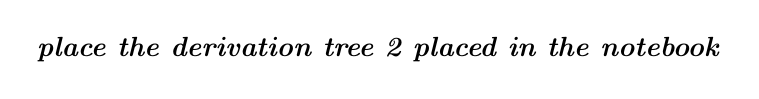
\begin{tikzpicture}[
	every node/.style={draw=none}]
\node{\textit{\textbf{place the derivation tree 2 placed in the notebook}}};
\label{dt:registerReply}
\end{tikzpicture}

where $e_2$ is the reply message and $E_3=[E_2 \backslash e_2]$.

From the derivation tree above, the remaining list $E_2$ starts with the
assynchronous message \texttt{sendSituation(spo2Situation)}. Thus, when the
reliability definition \ref{eq:assyncMessageReliability} is applied over $E_2$,
it results into the following derivation tree

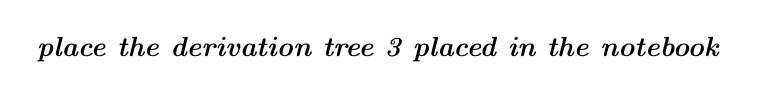
\begin{tikzpicture}
	[
		every node/.style={draw=none}
	]
\node{\textbf{\textit{place the derivation tree 3 placed in the notebook}}};
\label{dt:sndSituationAssync}
\end{tikzpicture}
where $e_2$ is the assynchronous message \texttt{sendSituation} and $E_3 =
[E_2 \backslash e_2]$ is the remaining list. 

The first element of the list $E_3$ is the synchronous message \texttt{persist}
directed to the software component responsible to persist data in different
manners. Thus, when the reliability definition~\ref{eq:syncMessageReliability}
is applied at $E_3$ it results into the following derivation tree

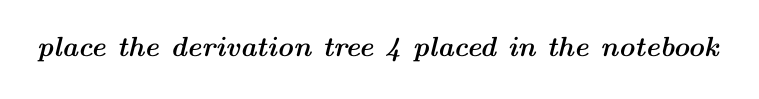
\begin{tikzpicture}
	[
		every node/.style={draw=none}
	]
\node{\textbf{\textit{place the derivation tree 4 placed in the notebook}}};
\label{dt:persistAssync}
\end{tikzpicture}

where $e_3$ is the assynchronous message and $E_4 = [E_3 \backslash e_3]$ is the list
containing the remaining elements after removing $e_3$ from $E_3$. 

The resulting list $E_4$ has as its first element the optional combined fragment
representing the behavior associated to the SQLite feature. According to the
reliability definition~\ref{eq:optionalFragmentReliability}, the reliability of the
optional fragment is represented by a single parameter, whose value will be
computed later. Since the element after the fragment representing the SQLite's
behavior is another combined fragment, for the sake of space, the derivation
tree shown below results from the twice application of
Definition~\ref{eq:optionalFragmentReliability} 

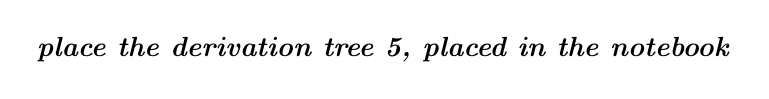
\begin{tikzpicture}
	[
		every node/.style={draw=none}
	]
\node{\textbf{\textit{place the derivation tree 5, placed in the notebook}}};
\label{dt:optSqliteMemory}
\end{tikzpicture}

where $e_6$ is the optional fragment associated to \texttt{SQLite} feature,
$E_6=[E_5 \backslash e_6 ]$, $e_7$ is the optional fragment associated to
\texttt{Memory} feature and $E_7 = [E_6 \backslash e_6]$ is the list containing
the remaining elements. 

At this point the $E_7$ list has the \texttt{reply} message (associated to
\texttt{persist} synchronous message) as its first element. Since the
reliability definition of a reply message is given by
\ref{eq:replyMessageReliability}, when it is applied it results into the
derivation tree

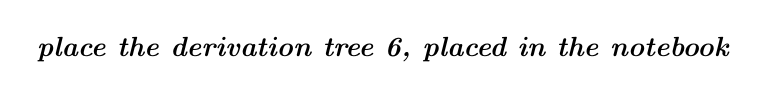
\begin{tikzpicture}
	[
		every node/.style={draw=none}
	]
\node{\textit{\textbf{place the derivation tree 6, placed in the notebook}}};
\label{dt:replyPersist}
\end{tikzpicture}

where $e_8$ is the reply message associated to the persist message and $E_8 =
[E_7 \backslash e_8]$ is the list of the remaining elements. 

At this point the $E_8$ contains the \texttt{sendSituation()} assynchronous
message as its first element, whose reliability definition is given by
\ref{eq:assyncMessageReliability}. Its application over the sequence diagram
results 

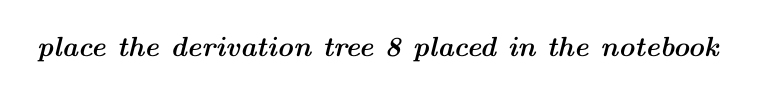
\begin{tikzpicture}
	[
		every node/.style={draw=none}
	]
\node{\textit{\textbf{place the derivation tree 8 placed in the notebook}}};
\label{dt:sndSituationAssync2}
\end{tikzpicture}

where $e_{10}$ is the reply message and $E_{10} = [E_9 \backslash e_{10}]$ is
the set of remaining elements after removing $e_{10}$ from $E_9$. 

Finally, the last iteration of the reliability function $R$ is over $E_{10}$
which is an empty list since all elements were already addressed. As the empty
list has no associated behavior, its reliability is $1.0$ by definition. Thus,
the derivation tree for $E_{10}$ is

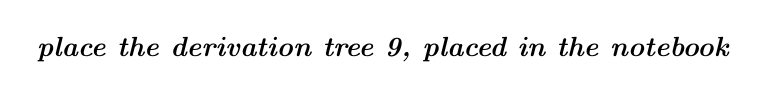
\begin{tikzpicture}
	[
		every node/.style={draw=none}
	]
\node{\textbf{\textit{place the derivation tree 9, placed in the notebook}}};
\label{dt:emptyList}
\end{tikzpicture}

Since there is no more element in the remaining elements list that represents
the sequence diagram, the resultant derivation tree is complete and it is shown
below.


\begin{tikzpicture}
	[
		every node/.style={draw=none}
	]
\node{\textbf{\textit{place the whole derivation tree here.}}};
\label{dt:wholeDT}
\end{tikzpicture}

Since the sequence diagram's reliability is given by the cummulated reliability
of its first element, as stated by Definition~\ref{}, it can be computed by
traversing the derivation tree~\ref{dt:wholeDT} in a pre-order fashion. Thus,
the result for such traversal is 
\begin{align}
R(Oxygenation) = &0.999 \times 0.999 \times 0.999 \times 0.999 \times rSqlite
\times \nonumber \\ &rMem \times 0.999 \times 0.999 \times 0.999 \nonumber \\
               = &0.999^7 \times rSqlite \times rMem
\label{eq:situationActivityDiagramReliability}
\end{align}

where the $rSqlite$ and $rMem$ are the variables that represent the
reliabilities of the optional fragments representing the behavior of SQLite and
Memory features, respectively.

Once \ref{eq:situationActivityDiagramReliability} is computed from the
reliability function $R$ applied at the activity diagram, it is necessary to
create its respective FDTMC by applying the transformation rules for sequence
diagram elements defined at
Section~\ref{sec:sequenceDiagramTransformationRules}. When the FDTMC building
is finished, its reliability can be computed by using the well-known reliability
definition provided by \cite{grunske_specification_2008} and the reachability
measure definition provided by \cite{baier_principles_2008}. 

The FDTMC building is accomplished in a stepwise fashion and follows the
partial-ordering of the set of sequence diagram elements. When an element is
transformed by its corresponding rule, its resulting FDTMC substructure is added
to the FDTMC created by previous transformation rules from the \textit{current state}. In the case of the "System
identifies \underline{situation}" sequence
diagram, the first element to be transformed is the \texttt{register}
synchronous message. When its transformation rule is applied (cf.
Figure~\ref{fig:transSync_SD}), the resulting FDTMC comprises the initial, error
and a new state besides two transitions, as shown by Figure \ref{xxx}.

\begin{figure}
\textbf{\textit{Place the FDTMC 1, depicted in the notebook.}}
\caption{FDTMC resulting from the transformation of \texttt{register} message.}
\label{fig:fdtmcRegister}
\end{figure}

The next element to be transformed, according to the sequence diagram's
partial-ordering is the \texttt{reply} message associated to the
\texttt{register} message. The transformation rules represented at
Figure~\ref{fig:trasReply_SD} builds a state and two edges newly created from
the current state, so results into the FDTMC shown by
Figure~\ref{fig:fdtmcRegisterReply}.

\begin{figure}
\textbf{\textit{Place the FDTMC 2, depicted in the notebook.}}
\caption{FDTMC resulting from the transformation of \texttt{reply} message.}
\label{fig:fdtmcRegisterReply}
\end{figure}

In the sequence, the \texttt{sendSituation} assynchronous message is transformed
into an FDTMC from the current state by the transformation rule represented at
Figure~\ref{fig:transAssync_SD}. The transformation adds a state and two states
newly created, as shown by Figure~\ref{fig:fdtmcSendSituation}.

\begin{figure} 
	\textbf{\textit{Place the FDTMC 3, depicted in the notebook.}}
	\caption{FDTMC resulting from the transformation of
	\texttt{sendSituation} message.} 
	\label{fig:fdtmcSendSituation}
\end{figure}

The next element to transform is the synchronous message \texttt{persist}. So
when its transformation is applied a state and two new edges are added from the
current state, that results the FDTMC shown by Figure~\ref{fig:fdtmcPersistSync}.

\begin{figure} 
	\textbf{\textit{Place the FDTMC 4, depicted in the notebook.}}
	\caption{FDTMC resulting from the transformation of \texttt{persist}
	message.} 
	\label{fig:fdtmcPersistSync}
\end{figure}

The next element to be transformed is the optional combined fragment
representing the behavior of SQLite feature. According to
Figure~\ref{fig:transOptFrag_SD} the transformation adds a state and two edges
newly created. The reliability of the fragment's internal sequence diagram is
represented on both created edges by the \texttt{rSqlite} variable, whose value
will be evaluated later. Since the next element is another optional combined
fragment that represents the memory feature's behavior, the analogous rationale
is valid such the transformation represented by Figure~\ref{fig:transOptFrag_SD}
is applied again. The result of such transformations is represented by
Figure~\ref{fig:fdtmcSqliteMemory}, where the elements added by both
transformations are distinguished from the existing elements for being
represented in solid lines.

\begin{figure} 
	\textbf{\textit{Place the FDTMC 5, depicted in the notebook.}}
	\caption{FDTMC resulting from the transformation of \texttt{SQLite} and
	\texttt{Memory} optional combined fragments.}
	\label{fig:fdtmcPersistSync}
\end{figure}

The next element to transform is the reply message associated to the
\texttt{persist}
synchronous message. When the transformation represented at
Figure~\ref{fig:transReply_SD} is applied it results into the FDTMC represented
by the Figure~\ref{fig:fdtmcReplyPersist}.

\begin{figure} 
	\textbf{\textit{Place the FDTMC 6, depicted in the notebook.}}
	\caption{FDTMC resulting from the transformation of \texttt{reply}
	message associated to the \texttt{persist} message.}
	\label{fig:fdtmcReplyPersist}.
\end{figure}

In the following the interaction between the \texttt{Oxygenation} and
\texttt{Bus} software components, comprised of the \texttt{sendSituation} and its return,
is transformed into a FDTMC substructure by applying the transformations for
\texttt{assynchronous} and \texttt{reply} message, in this sequence. The
resulting FDTMC is build by first adding a state and two edges newly created
from the current state, as defined by transformation of assynchronous rule
represented by Figure~\ref{fig:transAssync_SD}. From the new current state, the
FDTMC substructure corresponding to the reply message is build, by adding a
state and two newly created edges. As there is no other element to be
transformed, the current state is considered the FDTMC's last state to be reach
in case no error occur during the execution. Thus, it is labeled as ``success''
and transformed into an absorbing state by the auto-edge with $1.0$ as the
probability value. The Figure~\ref{fig:fdtmcSndSituationReply} is the final
FDTMC for the ``System identifies situation'' sequence diagram. 

\begin{figure} 
	\textbf{\textit{Place the FDTMC 7, depicted in the notebook.}}
	\caption{FDTMC resulting from the transformation of
		\texttt{sendSituation} and its corresponding \texttt{reply}
		message.}
	\label{fig:fdtmcReplyPersist}.
\end{figure}









For such FDTMC it is possible to apply the reachability measure
algorithm\cite{baier_principles_2008} in order to compute its
reliability\cite{grunske_specification_2008}. As
the FDTMC is comprised of a unique path from the \texttt{initial} to the
\texttt{sucess} state, the evaluation of the reliability property
$P=\Diamond(``sucess'')$ of the whole sequence diagram is equal to the
product of all probabilities along the path, including the parameters that
represent the reliabilities of the optional combined fragments.
Thus, such evaluation results into the following formula.

\scriptsize
\begin{align}
rOxygenation =&0.999 \times 0.999 \times 0.999 \times 0.999 \times rSqlite \times
rMemory \times 0.999 \times 0.999 \times 0.999 \times 0.999 \nonumber \\
rOxygenation =&0.999^7 \times rSQLite \times rMemory
\label{eq:oxygenationFDTMCReliability}
\end{align}
\normalsize

Given that \ref{eq:captureFDTMCReliability} denotes the reliability computed
from the FDTMC built from the transformation of the sequence diagram associated
to the ``System identifies situation'' activity, it is possible to analyse the
equivalence intuition depicted by
Figure~\ref{fig:reliabilityEquivalenceIntuition} in order to gather some
evidence concerning the reliabilities equivalence. In a brief, the sequence
diagram's reliability was computed by applying the reliability definitions for
each element in a stepwise fashion, which results into the reliability
formula~\ref{eq:situtationActivityDiagramReliability}. By the other side, the
sequence diagram was transformed into a FDTMC by applying the transformation
rules shown at Section~\ref{sec:sequenceDiagramTransformationRules}. The FDTMC
was evaluated by a well-known reachability algorithm which resulted the
formula~\ref{eq:oxygenationFDTMCReliability}. Both reliability formulae are
equals albeit they were computed using different methods, which provides the
evidence that the reliability of a sequence diagram and its FDTMC are
equivalent. In addition, as the FDTMC is build based on the transformation rules
and the FDTMC's reliability is equivalent to the sequence diagram's reliability,
it also provides the confidence that the transformation rules employed are also
correct.

Finally, it is important mention the behavioral variability of the ``System
identifies situation'' and its impact over its reliability. The behavior of
such sequence diagram is variable according to the optional combined fragments
which it comprises. By your turn, each combined fragment will only be executed
for the configurations which satisfy its guard condition. Thus, every time one
of its optional combined fragment is executed, its respective variable in the
formula~\ref{eq:oxygenationFDTMCReliability} assumes its reliability value. In
case its guard condition is not satisfied, its impact over the reliability of
the whole sequence diagram is null and, as the reliability given by
\ref{eq:captureFDTMCReliability} is a formula whose terms are products of of
reliabilities, its respective variable assumes $1.0$ as reliability value so it
does not affect the reliability computation. 
